\documentclass{article}

\usepackage{fancyhdr}
\usepackage{extramarks}
\usepackage{amsmath}
\usepackage{amsthm}
\usepackage{amsfonts}
\usepackage{tikz}
\usepackage[plain]{algorithm}

\usetikzlibrary{automata,positioning}
\usepackage{titling}
\usepackage{chngcntr}
\counterwithin{figure}{section}
\usepackage{sectsty}
\sectionfont{\fontsize{15}{15}\selectfont}
\usepackage{multirow}
\usepackage{booktabs}
\usepackage{arydshln}
\usepackage[font={scriptsize}]{caption}
\usepackage{listings}
\usepackage{color}
\usepackage{subfigure}
\usepackage{subfig}
\definecolor{mygreen}{RGB}{28,172,0} 
\definecolor{mylilas}{RGB}{170,55,241}
%
% Basic Document Settings
%

\topmargin=-0.45in
\evensidemargin=0in
\oddsidemargin=0in
\textwidth=6.5in
\textheight=9.0in
\headsep=0.25in

\linespread{1.1}

\pagestyle{fancy}
\lhead{\hmwkClass}
\rhead{\hmwkTitle}
\cfoot{\thepage}

\renewcommand\headrulewidth{0.4pt}
\renewcommand\footrulewidth{0.4pt}
\renewcommand{\thesubsubsection}{\alph{subsubsection})}
\setlength\parindent{0pt}

\lstdefinestyle{matlab}{
	language=Matlab,%
    basicstyle=\scriptsize,
    breaklines=true,%
    morekeywords={matlab2tikz},
    keywordstyle=\color{blue},%
    morekeywords=[2]{1}, keywordstyle=[2]{\color{black}},
    identifierstyle=\color{black},%
    stringstyle=\color{mylilas},
    commentstyle=\color{mygreen},%
    showstringspaces=false,%without this there will be a symbol in the places where there is a space
    %numbers=left,%
    %numberstyle={\tiny \color{black}},% size of the numbers
    %numbersep=9pt, % this defines how far the numbers are from the text
    emph=[1]{for,end,break},emphstyle=[1]\color{red}, %some words to emphasise
    %emph=[2]{word1,word2}, emphstyle=[2]{style},    
}
%
% Homework Details
%   - Title
%   - Due date
%   - Class
%   - Section/Time
%   - Instructor
%   - Author
%

\newcommand{\hmwkTitle}{}
\newcommand{\hmwkDueDate}{}
\newcommand{\hmwkClass}{Sliding Mode Control of a PVTOL system}
\newcommand{\hmwkClassTime}{}
\newcommand{\hmwkClassInstructor}{}
\newcommand{\hmwkAuthorName}{}
\newcommand{\hmwkAuthorEmail}{Subodh.Mishra.eleves@ec-nantes.fr}
\newcommand{\figurescaling}{width=\textwidth}


\begin{document}
\clearpage
\thispagestyle{empty}
\clearpage
\noindent\rule{\textwidth}{0.4pt} \\
\textbf{\MakeUppercase{\hmwkClass}} \\
\textbf{\MakeUppercase{\hmwkTitle}} \\
\hmwkDueDate \\
%-----------------------------------TOP PAGE-----------------------------

\noindent\rule{\textwidth}{0.4pt}
\section{System description}
\textbf{PVTOL} stands for \textbf{P}lanar \textbf{V}ertical \textbf{T}ake\textbf{o}ff and \textbf{L}anding. In this report, the sliding mode control of a PVTOL system landing is studied. The planar aircraft studied here has a minimum number of states and inputs but has many of the features that must be considered while designing control laws for real PVTOL systems. The  aircraft state is simply the position, $x$, $z$ of the aircraft centre of mass, the roll angle of the craft $\theta$ and the corresponding velocities $\dot{x}$, $\dot{z}$ and $\dot{\theta}$. The control inputs $u_1$, $u_2$, are the thrust and the rolling moment. \\
\begin{figure}[H]
\centering
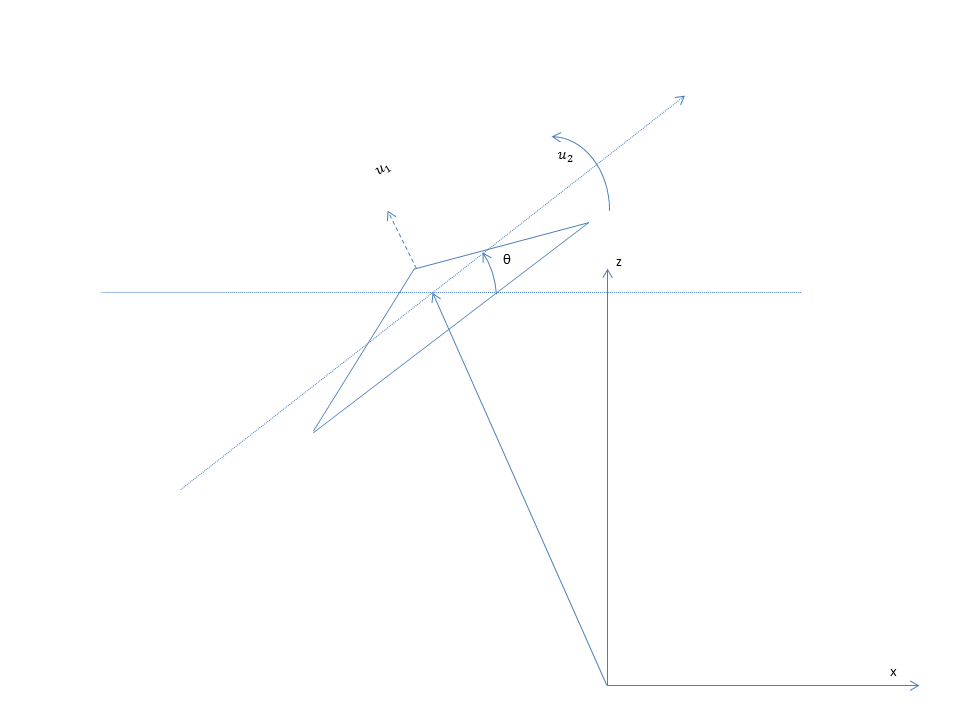
\includegraphics[width = 0.8\textwidth]{Figures/figure1.png}
\caption{The PVTOL Aircraft}
\label{fig:figure1}
\end{figure}
\section{System Equations}
The equations of motion of the above PVTOL aircraft are:
\begin{equation}\label{set 1.1}
  \begin{split}
\ddot{x}&=-u_1 \sin \theta \\
\ddot{z}&=u_1 \cos \theta -1\\
\ddot{\theta}&=u_2 + \delta(t)
  \end{split}
\end{equation}
$\delta(t)$ is a disturbance input or uncertianity.\\
The control objective is to stabilize $[x,z]^T$ at $[0,0]^T$.\\
The system outputs are $x$ and $z$. Differentiating the model system outputs, $x$ and $z$, we get:


\begin{align}
\left[\begin{array}{cc}\ddot{x}\\\ddot{z}\end{array}\right] &= \left[\begin{array}{c}0\\1\end{array}\right] + \left[\begin{array}{cc}-\sin\theta & 0\\\cos \theta &0 \end{array}\right] \left[\begin{array}{c}u_1\\u_2\end{array}\right] \label{set 1.2}
\end{align}\begin{figure}[H]
\centering
\includegraphics[width = 0.8\textwidth]{Figures/openloop.png}
\caption{Simulink Model of PVTOL system controlled using Sliding Mode Control }
\label{fig:figure2}
\end{figure}


Clearly, $u_2$ has no effect on this system. As $u_2$ comes into the system only through $\ddot{\theta}$, the Equation \ref{set 1.2} needs to be differentiated at least two more times and the following results:
\begin{align}
\left[\begin{array}{cc}x^{(4)}\\z^{(4)}\end{array}\right] &= \left[\begin{array}{c}
\sin \theta \dot{\theta}^2u_1-2\cos \theta \dot{\theta}\dot{u}_1
\\-\cos \theta \dot{\theta}^2u_1-2\sin \theta \dot{\theta}\dot{u}_1
\end{array}\right] + \left[\begin{array}{cc}-\sin\theta & -\cos \theta u_1\\
\cos \theta &-\sin \theta u_1 \end{array}\right] \left[\begin{array}{c}\ddot{u}_1\\u_2\end{array}\right] \label{set 1.3}
\end{align}
As evident from Equation \ref{set 1.3}, the system takes $[\ddot{u}_1,u_2]^T$ as input.
Without loss of generality, the disturbance can be set to zero for the derivation of Equation \ref{set 1.3}.
\section{Sliding Mode Control}
\label{SMC}
The first step is to choose a sliding variable which has a relative degree one with respect to the system inputs. As Equation \ref{set 1.3} involves $4^{th}$ order derivative, the sliding variable should be:

\begin{align}
\left[\begin{array}{cc}s_1\\s_2\end{array}\right] &= \left[\begin{array}{cc}x^{(3)}\\z^{(3)}\end{array}\right] + a\left[\begin{array}{cc}\ddot{x}\\\ddot{z}\end{array}\right] + b\left[\begin{array}{cc}\dot{x}\\\dot{z}\end{array}\right] + c\left[\begin{array}{cc}{x}\\{z}\end{array}\right]  
 \label{set 1.4}
\end{align}
Differentiating once with respect to time:
\begin{align*}
\left[\begin{array}{cc}\dot{s}_1\\\dot{s}_2\end{array}\right] &= \left[\begin{array}{cc}x^{(4)}\\z^{(4)}\end{array}\right] + a\left[\begin{array}{cc}x^{(3)}\\z^{(3)}\end{array}\right] + b\left[\begin{array}{cc}\ddot{x}\\\ddot{z}\end{array}\right] + c\left[\begin{array}{cc}\dot{x}\\\dot{z}\end{array}\right]  
\ 
\end{align*}
Using Equation \ref{set 1.3}:
\begin{align}
\left[\begin{array}{cc}\dot{s}_1\\\dot{s}_2\end{array}\right] &= \left[\begin{array}{c}
\sin \theta \dot{\theta}^2u_1-2\cos \theta \dot{\theta}\dot{u}_1
\\-\cos \theta \dot{\theta}^2u_1-2\sin \theta \dot{\theta}\dot{u}_1
\end{array}\right] +a\left[\begin{array}{cc}x^{(3)}\\z^{(3)}\end{array}\right] + b\left[\begin{array}{cc}\ddot{x}\\\ddot{z}\end{array}\right] + c\left[\begin{array}{cc}\dot{x}\\\dot{z}\end{array}\right]+\left[\begin{array}{cc}-\sin\theta & -\cos \theta u_1\\
\cos \theta &-\sin \theta u_1 \end{array}\right] \left[\begin{array}{c}\ddot{u}_1\\u_2\end{array}\right] 
\ \label{set 1.5}
\end{align}
It can be noted that the sliding variable has  a relative degree 1 with respect to the inputs  $[\ddot{u}_1,u_2]^T$.\\

The control objective is to ensure:
\begin{align}
s&=0
\label{set 1.6}
\end{align}
Using Equations \ref{set 1.4} and \ref{set 1.6} we can conclude that $a$,$b$ and $c$ must be chosen such that the characteristic equation formed by $s=0$ has roots with negative real part. An easy and practical method is to choose all the poles to be real,equal and negative(critically damped system). For this report the value of the pole is chosen to be $-3$ and this helps to determine $a$,$b$ and $c$. 

\begin{align*}
(s+3)^3=s^3+as^2+bs+c
\end{align*}

This yeilds:

\begin{equation}\label{set 1.7}
  \begin{split}
  a&=9 \\
  b&=27\\
  c&=27
  \end{split}
\end{equation}
Let $\alpha(x,t)$ be defined as:
\[ \alpha(x,t)= \left[\begin{array}{c}
\sin \theta \dot{\theta}^2u_1-2\cos \theta \dot{\theta}\dot{u}_1
\\-\cos \theta \dot{\theta}^2u_1-2\sin \theta \dot{\theta}\dot{u}_1
\end{array}\right] +a\left[\begin{array}{cc}x^{(3)}\\z^{(3)}\end{array}\right] + b\left[\begin{array}{cc}\ddot{x}\\\ddot{z}\end{array}\right] + c\left[\begin{array}{cc}\dot{x}\\\dot{z}\end{array}\right]\]
and $\beta(x,t)$ is defined as:
\[ \beta(x,t)= \left[\begin{array}{cc}-\sin\theta & -\cos \theta u_1\\
\cos \theta &-\sin \theta u_1 \end{array}\right] \]
\textbf{Note:} Here, $x$ refers to the states of the system $[x,\dot{x},y,\dot{y},\theta ,\dot{\theta},u_1,\dot{u}_1 ]$ and $t$ refers to time.
Writing Equation \ref{set 1.5} by including effects of disturbances, one gets:

\begin{align}
\dot{s}=\alpha(x,t)+\beta(x,t)u+\Delta(t)
\label{set 1.8}
\end{align}
where:
\begin{align*}
u=\left[\begin{array}{c}\ddot{u}_1\\u_2\end{array}\right] 
\ 
\end{align*}
$\alpha(x,t)$ and $\beta(x,t)$ are known and bounded. For this example we consider the disturbance $\Delta(t)$ to be bounded.

For sliding to occur along $s=0$, the controller must not only linarize the system defined by Equation \ref{set 1.8} but also nullify the effects of the disturbance $\Delta(t)$. In fact, the controller must ensure $s\dot{s}<0$.\\
If, $u$ is chosen as:

\begin{align}
u=\beta^{-1}(x,t)\Big(-\alpha(x,t)+\left[\begin{array}{cc}-K_x.sign(s_1)\\-K_z.sign(s_2)\end{array}\right]\Big) 
\label{set 1.9}
\end{align}

Using Equations \ref{set 1.8} and \ref{set 1.9}:
\begin{align}
\dot{s}=\left[\begin{array}{cc}-K_x.sign(s_1)\\-K_z.sign(s_2)\end{array}\right]+\Delta(t)
\label{set 1.10}
\end{align}
To satisfy $s\dot{s}<0$, $K_x$ and $K_y$ must be postive and sufficiently larger than the maximum amplitude of the disturbance $|\Delta_M|$. This is a demerit of the present approach because one needs to know the bounds of the disturbance. \\
\begin{figure}[H]
\centering
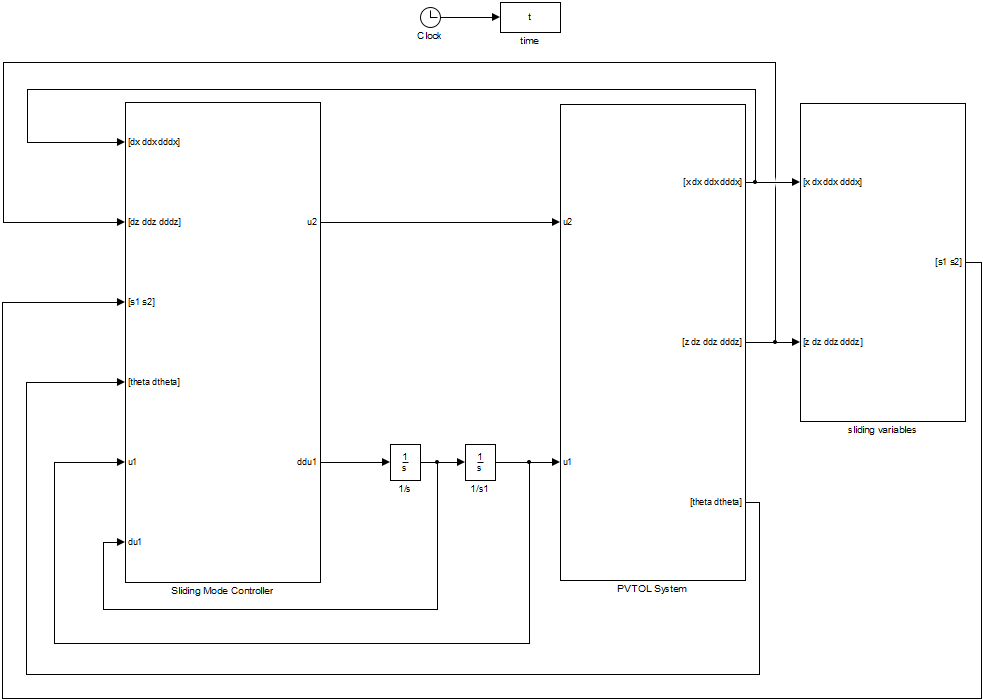
\includegraphics[width = 0.8\textwidth]{Figures/figure2.png}
\caption{Simulink Model of PVTOL system controlled using Sliding Mode Control }
\label{fig:figure2}
\end{figure}
\textbf{Note:} The system is simulated in \texttt{Simulink  }using a fixed step \texttt{Runge Kutta Solver}. The inital conditions for $[x,y,\theta]^T=[2,1,0]^T$\\
The given model is simulated for:
\begin{itemize}
\item \textbf{Disturbance: $\delta(t)=200\sin t$}\\
 The model is simulated for sufficiently high gains $K_x=600$ and $K_z=600$.
 
\begin{figure}[H]
\centering
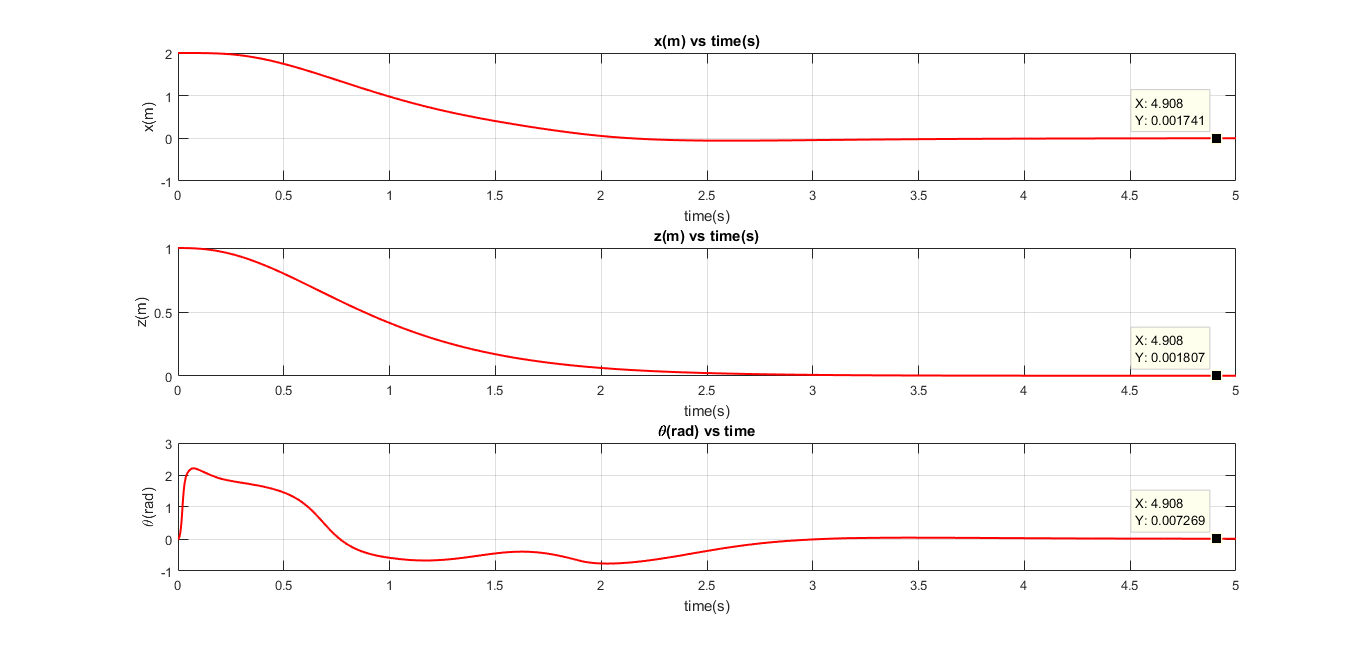
\includegraphics[width = 0.8\textwidth]{Figures/figure3.png}
\caption{Evolution of $x$,$z$ and $\theta$}
\label{fig:figure3}
\end{figure}

\begin{figure}[H]
\centering
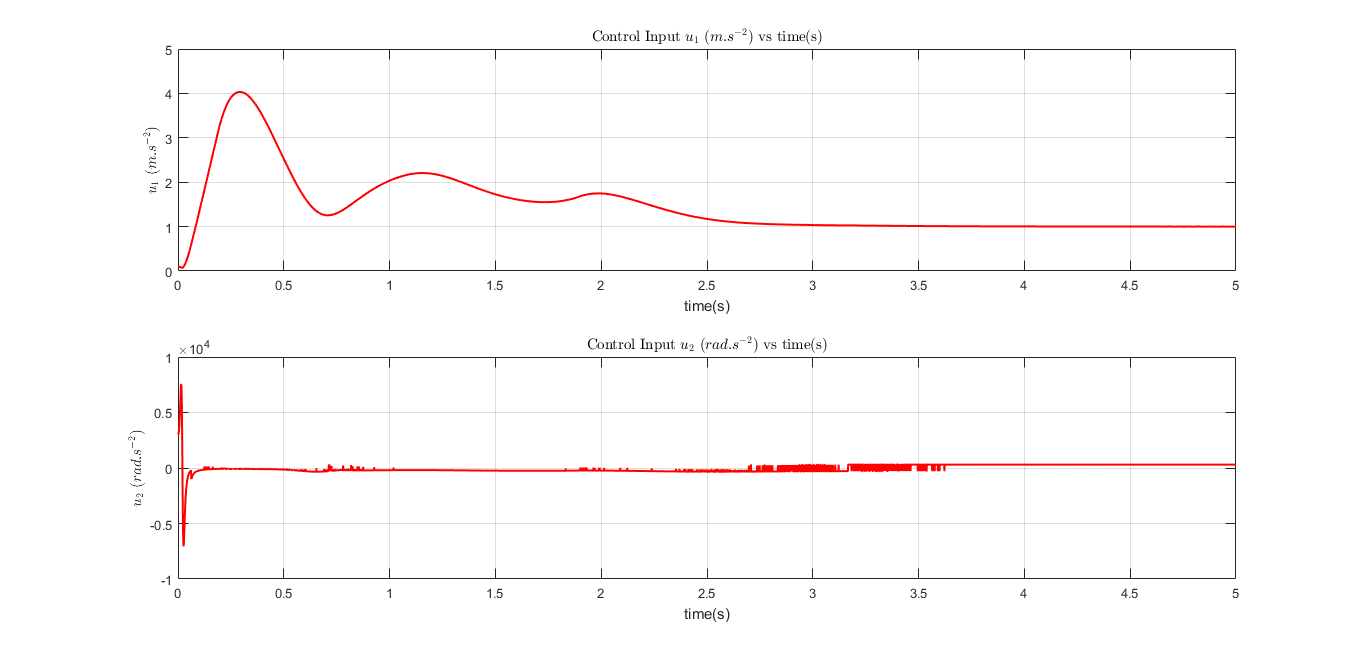
\includegraphics[width = 0.8\textwidth]{Figures/figure4.png}
\caption{Evolution of the control inputs $u_1$ and $u_2$}
\label{fig:figure4}
\end{figure}

\begin{figure}[H]
\centering
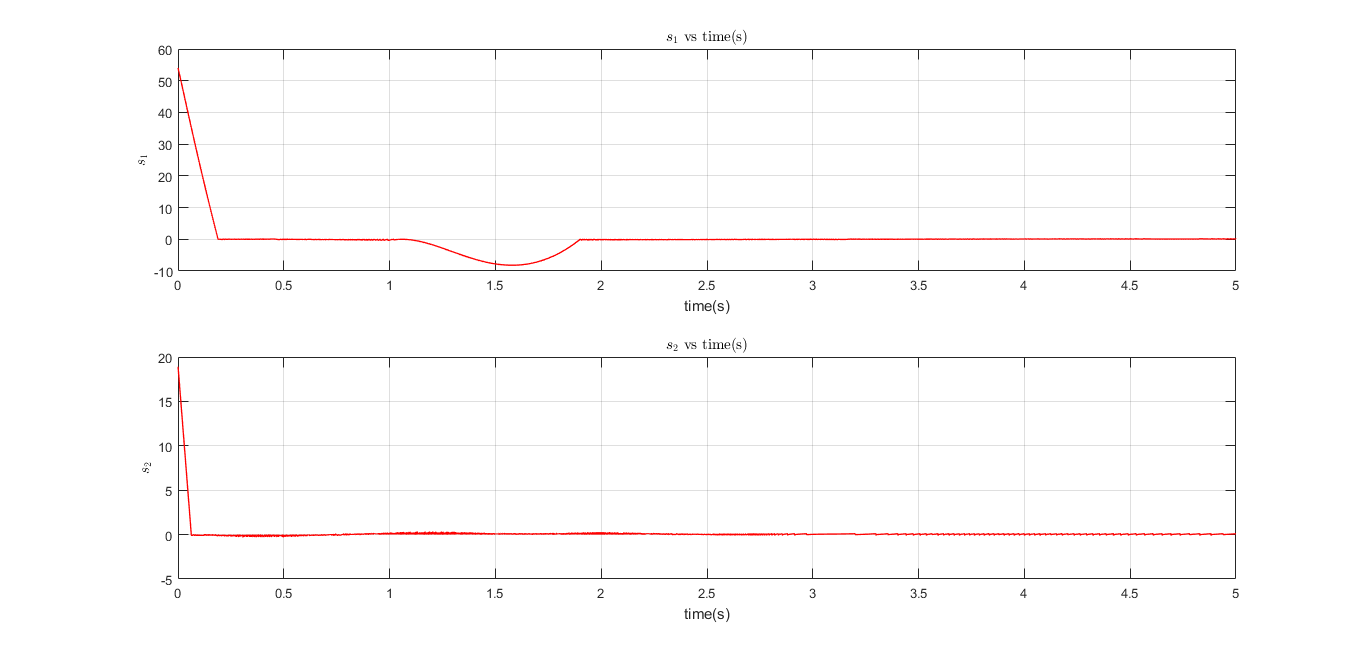
\includegraphics[width = 0.8\textwidth]{Figures/figure5.png}
\caption{Evolution of the sliding variables $s_1$ and $s_2$}
\label{fig:figure5}
\end{figure}
In Figure \ref{fig:figure3} it can be seen that $x$, $y$ and $z$ converge very near to zero. The control inputs are stable and bounded. In Figure \ref{fig:figure4}, $u_1$ converges to 1 and $u_2$ switches frequently but is bounded. The sliding variables are shown in \ref{fig:figure5} and the chatter in $s_2$ is more prominent. $x$,$y$ and $\theta$ converge very near to zero in approximately 3 seconds.
\item \textbf{Disturbance: $\delta(t)=200$}\\
The model is simulated with $K_x=800$ and $K_z=800$. If the gains are very low then the system does not converge and becomes unstable.
\begin{figure}[H]
\centering
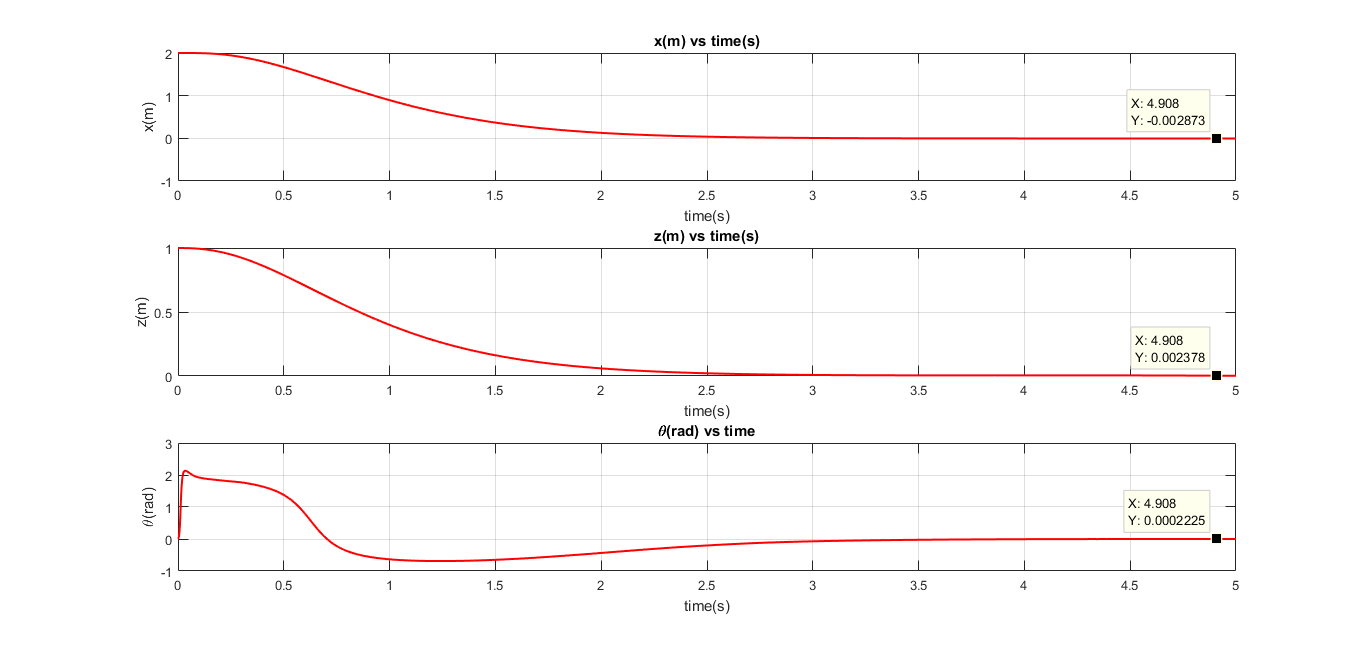
\includegraphics[width = 0.8\textwidth]{Figures/figure6.png}
\caption{Evolution of $x$,$z$ and $\theta$}
\label{fig:figure6}
\end{figure}

\begin{figure}[H]
\centering
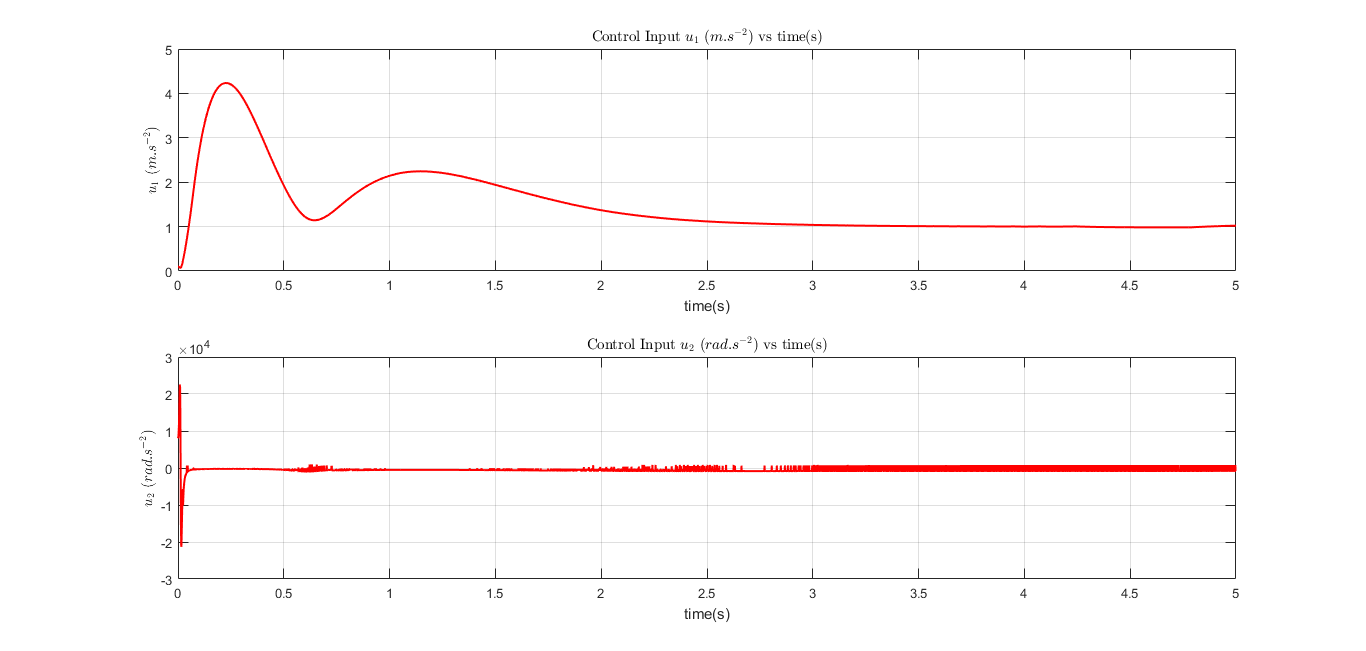
\includegraphics[width = 0.8\textwidth]{Figures/figure7.png}
\caption{Evolution of the control inputs $u_1$ and $u_2$}
\label{fig:figure7}
\end{figure}

\begin{figure}[H]
\centering
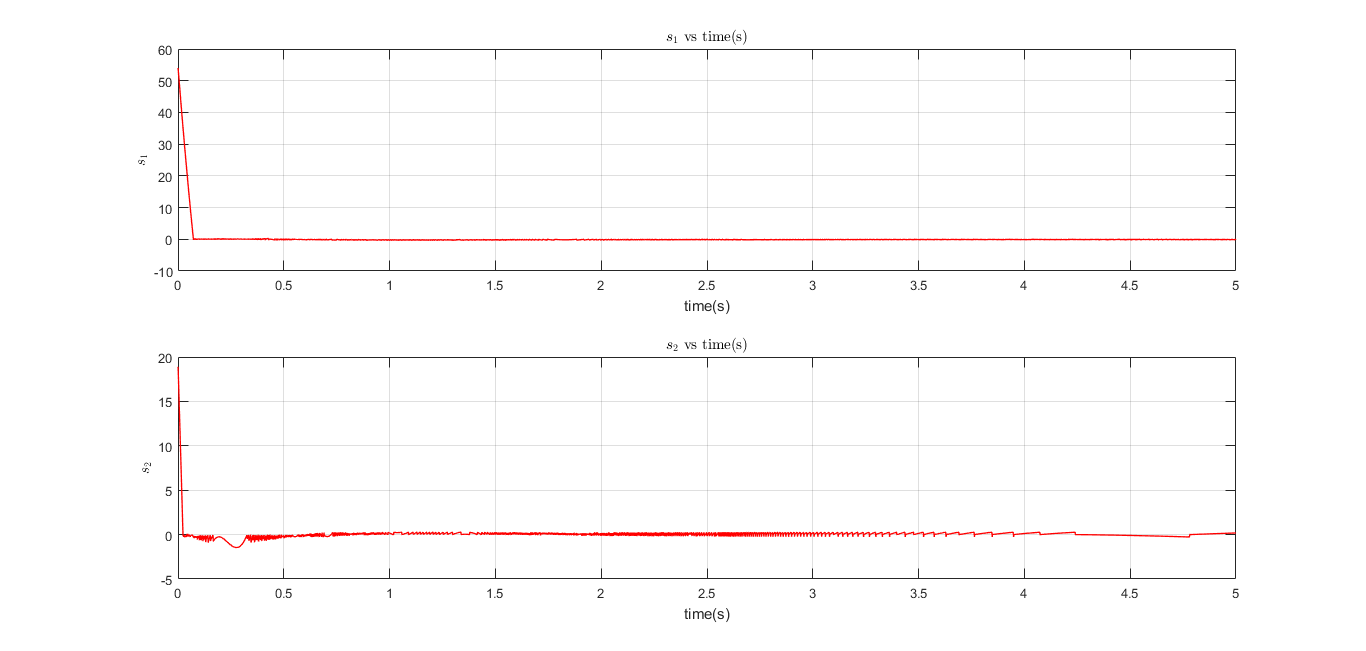
\includegraphics[width = 0.8\textwidth]{Figures/figure8.png}
\caption{Evolution of the sliding variables $s_1$ and $s_2$}
\label{fig:figure8}
\end{figure}

In Figure \ref{fig:figure6} it can be seen that $x$, $y$ and $z$ converge very near to zero. The control inputs are stable and bounded. In Figure \ref{fig:figure7}, $u_1$ converges to 1 and $u_2$ switches frequently but is bounded. The sliding variables are shown in \ref{fig:figure8} and the chatter in $s_2$ is more prominent. $x$,$y$ and $\theta$ converge very near to zero in approximately 2.5 seconds. The chatter in the control inputs and sliding variables is more in this case than in the case where the disturbance is a sinusoid. But, for both the cases the amplitude of disturbance is known and the gains must be definitely larger than the disturbance amplitude to ensure stability and convergence.
\end{itemize}
\section{Adaptive Sliding Mode Control}
The demerit of the Sliding Mode Control described in Section \ref{SMC} is, the prior knowledge of the amplitude of the disturbance is required to determine the magnitude of the controller gains. Moreover, after the sliding condition is attained, there is absolutely no need to use high gains. After sliding is obtained, the gain must be high enough to counter the disturbances and perturbations. In this adaptive sliding mode control the gain evolves over time and starts reducing once sliding condition is approached. 
A brief description of this algorithm follows.
\subsection{Algorithm} 
The objective of this algorithm consists in using a dynamical gain which will be adapted, online, with respect to the establishment(or not) of a sliding motion. Let the control be $v=[v_1,v_2]^T$ and $s=[s_1,s_2]^T$ be the sliding variable(s),then:\\

\begin{equation}\label{set 1.11}
  \begin{split}
   v_1&=-K_x.sign(s_1) \\
   v_2&=-K_y.sign(s_2)  
  \end{split}
\end{equation}
with the gain $K_i(t)$ defined such that:
\begin{align}
\begin{split}\label{set 1.12}
\dot{K}_i & = \begin{cases}\bar{K}_i|s_i|\mathrm{sign}(|s_i| - \mu_i)\qquad &K_i > \eta_i\\\eta_i &K_i\leq \eta_i\end{cases}
\end{split}
\end{align}
with $i\in\{x,y\}$, $K_i(0)>0$,$\bar{K}_{i}>0$,$\eta_i>0$ and $\mu_i>0$ very small.
\subsection{Working}
A $\mu$ band is cosidered in this case. This band is defined as:

\begin{align}
|s_i|<\mu_i 
\label{set 1.13}
\end{align}
Once the sliding variable $s$ reaches inside this band, by Equation \ref{set 1.12}, $\dot{K}_i$ will be negative, so, the gain will start reducing gradually. But, it cannot decrease indefinitely, according to the condition imposed by Equation \ref{set 1.12}, it can only decrease till its value equals $\eta_i$. This makes sure that the gain reduces on approaching the sliding surface and maintains a value that it enough to counter the effects of disturbances and uncertainities.\\
$\mu_i$ is a like a threshold value. If $|s|$ is below this threshold then gain reduces. If it is outside this threshold then the gain keeps on increasing.
\subsection{Simulation}
\subsection{Tuning $\mu$}
If $\mu$ is not properly tuned then the system may become unstable and the control gains may increase indefinity. If the parameter $\mu$ is too small then the $\mu$ band will be very narrow , if, at the same time, the gain  and the sampling period is relatively high, then the trajectory of $s$ will be such that it will never stay within the $\mu$ band, consequently, $\dot{K}_i$ will always be positive, resulting in increase in $K_i$ to infinitely large values. Such high gains will induce larger oscillations and result in divergence. In this case, the solution could be, reduction of the sampling time or the gain (by reducing $\bar{K}_i$ and $\eta_i$) or both. Another solution could be, increasing $\mu_i$.\\
If the parameter $\mu$ is too large, it implies that the $\mu$ band is too large and this means that the gain will start reducing even is the sliding variable is far away from the sliding surface. This is detrimental because he controller accuracy will not be as good as required. But, this will not bring in any instabillity even if the accurcy is bad.\\
So, the minimum admissible value of $\mu$ depends on the gain and the sampling period and it needs to be tuned to a higher value if one or both of them is high and vice versa.
\end{document}